\documentclass[pdf]{beamer}
\usepackage[utf8]{inputenc}
\usepackage{graphicx}
\usepackage[export]{adjustbox}

\mode<presentation>{\usetheme{Warsaw}}
\setbeamertemplate{footline}[frame number]
\AtBeginSection[]
{
\begin{frame}{Table of Contents}
\tableofcontents[currentsection]
\end{frame}
}

\title{\textbf{An FPGA Implementation of a \\ Digital Storage Oscilloscope}}
\author{
    Andrei Purcarus \and Ze Yu Yang
}
\institute{
	ECSE 487 \\
	McGill University
}
\date{April 10, 2017}

\begin{document}

\maketitle

\begin{frame}
\frametitle{Table of Contents}
\tableofcontents
\end{frame}

\section{Introduction}

\begin{frame}
\frametitle{Objectives}
\begin{itemize}
\item Display of waveforms with frequencies from 1~kHz to 200~kHz
\item Frequency measurements with an accuracy of 1~\%~+~10~Hz
\item Voltage measurements with an accuracy of 1~\%~+~10~mV
\end{itemize}
\end{frame}

\section{Design Methodology}

\begin{frame}
\frametitle{System}
\begin{figure}[!htb]
  \includegraphics[width=\linewidth]{diagrams/system.pdf}
\end{figure}
\end{frame}

\begin{frame}
\frametitle{VGA Driver}
\begin{figure}[!htb]
  \includegraphics[width=\linewidth]{diagrams/vga_driver.pdf}
\end{figure}
\end{frame}

\begin{frame}
\frametitle{Triggering}
\begin{figure}[!htb]
  \includegraphics[width=\linewidth]{diagrams/triggering.pdf}
\end{figure}
\end{frame}

\begin{frame}
\frametitle{Data Acquisition}
\begin{figure}[!htb]
  \includegraphics[height=0.8\textheight]{diagrams/data_acquisition.pdf}
\end{figure}
\end{frame}

\begin{frame}
\frametitle{Sin(x)/x Interpolation}
\begin{figure}[!htb]
  \includegraphics[width=\linewidth]{diagrams/sinc_interpolation.pdf}
\end{figure}
\end{frame}

\begin{frame}
\frametitle{Trigger Correction}
\begin{figure}[!htb]
  \includegraphics[width=\linewidth]{diagrams/trigger_correction.pdf}
\end{figure}
\end{frame}

\begin{frame}
\frametitle{ADC Interface}
\begin{figure}[!htb]
  \includegraphics[width=\linewidth]{diagrams/adc_interface.pdf}
\end{figure}
\end{frame}

\section{Results}

\begin{frame}
\frametitle{Triggering}
\begin{figure}[!htb]
  \includegraphics[width=\linewidth]{test-results/trigger_test_rising_10kHz.png}
\end{figure}
\begin{figure}[!htb]
  \includegraphics[width=\linewidth]{test-results/trigger_test_falling_200kHz.png}
\end{figure}
\end{frame}

\begin{frame}
\frametitle{Data Acquisition}
\begin{figure}[!htb]
  \includegraphics[width=\linewidth]{test-results/data_acquisition_test.png}
\end{figure}
\end{frame}

\begin{frame}
\frametitle{Oscilloscope}
\begin{figure}[!htb]
  \includegraphics[height=0.8\textheight]{test-results/scope_demo_1kHz.png}
\end{figure}
\end{frame}

\begin{frame}
\frametitle{Oscilloscope}
\begin{figure}[!htb]
  \includegraphics[height=0.8\textheight]{test-results/scope_demo_10kHz.png}
\end{figure}
\end{frame}

\begin{frame}
\frametitle{Oscilloscope}
\begin{figure}[!htb]
  \includegraphics[height=0.8\textheight]{test-results/scope_demo_100kHz.png}
\end{figure}
\end{frame}

\begin{frame}
\frametitle{Oscilloscope}
\begin{figure}[!htb]
  \includegraphics[height=0.8\textheight]{test-results/scope_demo_200kHz.png}
\end{figure}
\end{frame}

\begin{frame}
\frametitle{Synthesis}
\begin{table}[!htb]
    \centering
    \begin{tabular}[c]{ | l | l | }
    	\hline
        \textbf{Family} & Cyclone V \\
        \hline
        \textbf{Device} & 5CSEMA5F31C6 \\
        \hline
        \textbf{Logic Utilization} & 19,901 / 32,070 ( 62~\% ) \\
        \hline
        \textbf{Total Registers} & 23770 \\
        \hline
        \textbf{Total Block Memory Bits} & 246,832 / 4,065,280 ( 6 \% ) \\
        \hline
        \textbf{Total DSP Blocks} & 87 / 87 ( 100 \% ) \\
        \hline
        \textbf{Fmax} & 60.26~MHz \\
        \hline
        \textbf{Setup Slack} & 3.405~ns \\
        \hline
        \textbf{Hold Slack} & 0.016~ns \\
        \hline
    \end{tabular}
\end{table}
\end{frame}

\begin{frame}
\frametitle{Frequency Measurement Error}
\begin{figure}[!htb]
  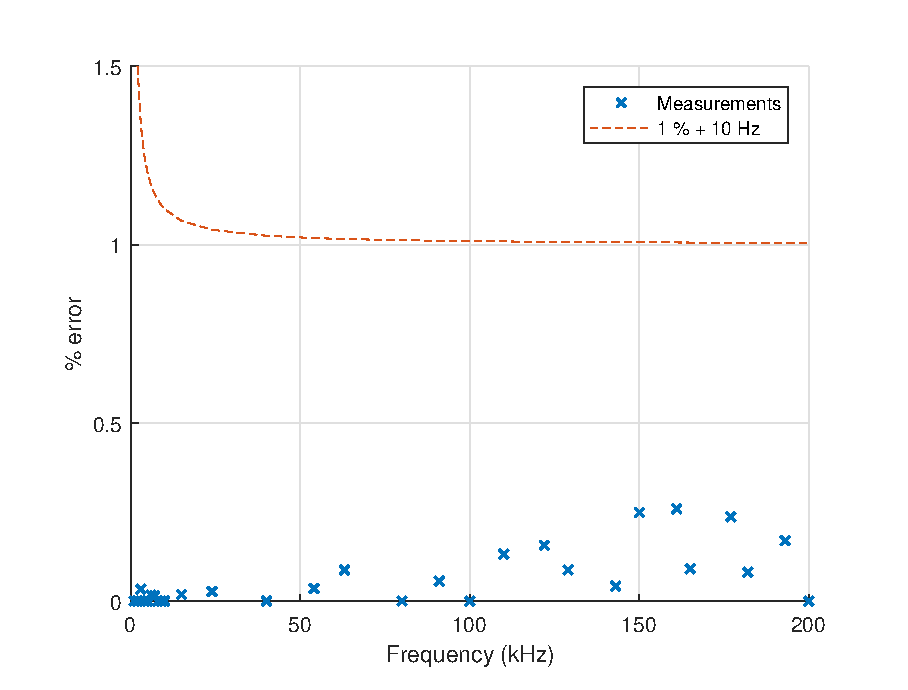
\includegraphics[height=0.8\textheight]{test-results/freq.eps}
\end{figure}
\end{frame}

\begin{frame}
\frametitle{Absolute Voltage Measurement Error}
\begin{figure}[!htb]
  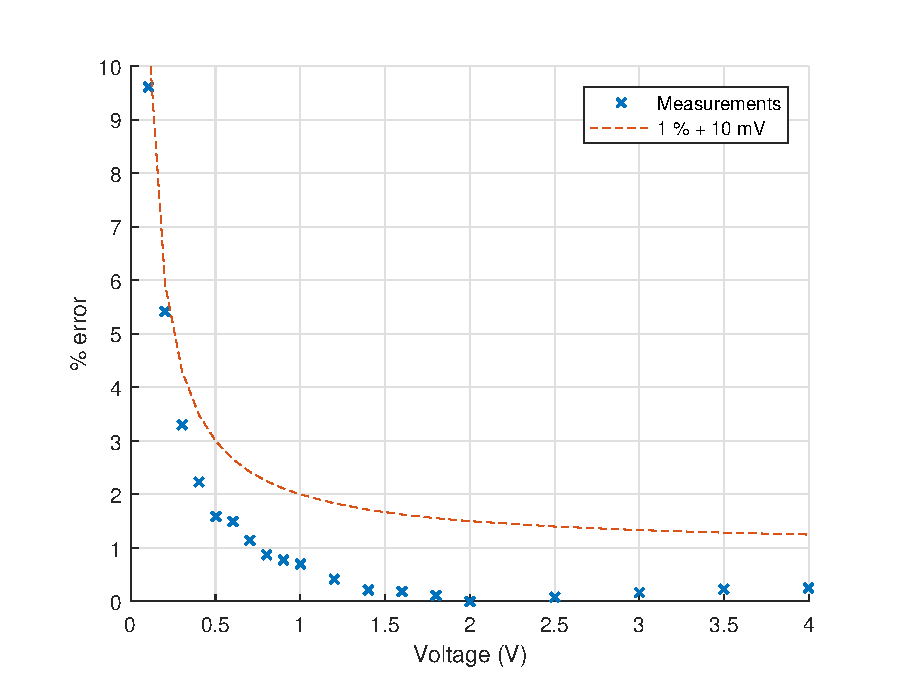
\includegraphics[height=0.8\textheight]{test-results/volt.eps}
\end{figure}
\end{frame}

\begin{frame}
\frametitle{Relative Voltage Measurement Error}
\begin{figure}[!htb]
  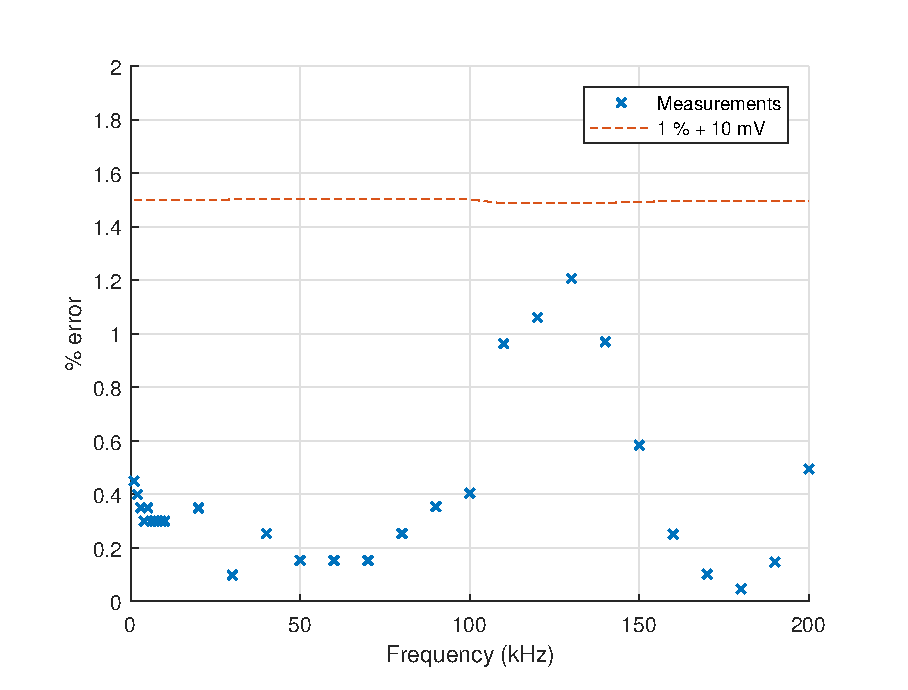
\includegraphics[height=0.8\textheight]{test-results/voltpp.eps}
\end{figure}
\end{frame}

\end{document}
